\documentclass[10pt]{article}

\usepackage{spheric}
%%%TITLE
\title{A development of a SPH model for simulation of abrasive-water-jet impacting on a metallic surface}
\date{}

%%AFFILIATIONS
\author[1,2]{Xiangwei Dong$^\dagger$}
\author[1]{Zengliang Li}
\author[2]{Jianlin Liu}


\affil[1]{College of mechanical and electronic engineering, China University of Petroleum (East China),
66 Changjiang Rd, Huangdao District, Qingdao, China}
\affil[2]{College of Pipeline and Civil Engineering, China University of Petroleum (East China),
66 Changjiang Rd, Huangdao District, Qingdao, China}
\affil[$\relax$]{\email{\dagger}{dongxw139@163.com}}


%%DOCUMENT
\begin{document}

\maketitle

%\SelectedTopics{}

%%PLEASE PUT YOUR ABSTRACT HERE
\begin{abstract}

A lagrangian model for the numerical simulation of the impact of abrasive water-jet on metallic surface is proposed in this paper. In the method both fluid and solid phases are described by smoothing particle hydrodynamics: water is modeled as a viscous fluid with weak compressibility, while metallic plate is modeled as an elastic-plastic material. Abrasive particles are modeled as rigid bodies with specified geometries. The interactions between fluid and solid, fluid and particles, particles and solid are realized by suitable terms, which are commonly used in the SPH method. Simulation tests of surface erosion by a water-jet containing single and multiple particles are carried out as challenging examples to verify the applicability of the SPH model. This supports the attractiveness of this new approach in relevant applications, such as solid particle erosion, abrasive water-jet machining, etc. Advantages of the method are robustness, conceptual simplicity and relative ease of incorporating new physics.


\begin{figure}[!htb]
\centering
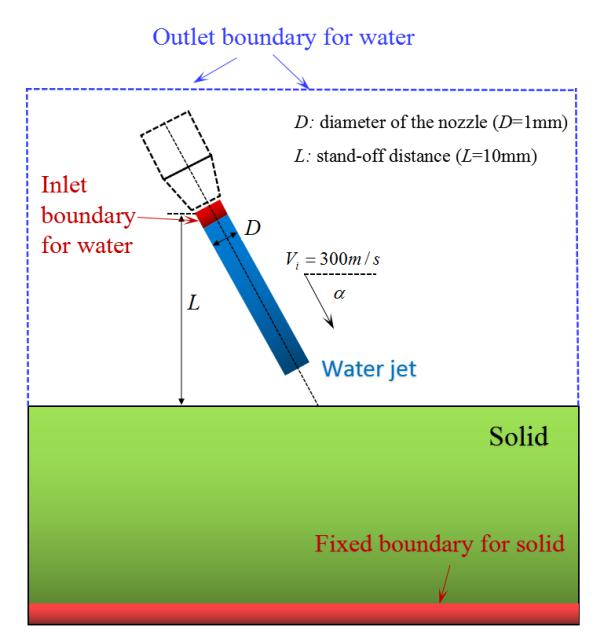
\includegraphics[width=0.46\textwidth]{47-11.png}~~~
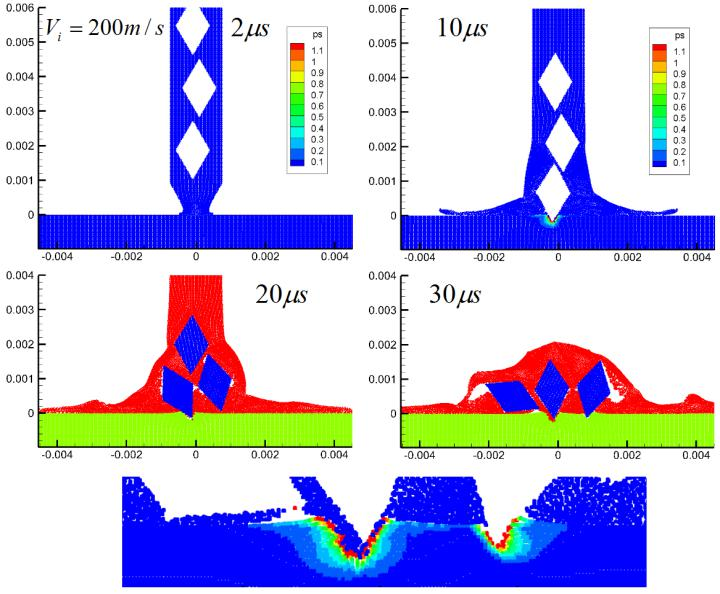
\includegraphics[width=0.46\textwidth]{47-12.png}~~~
\caption{Graphic abstract}\label{fig:47}
\end{figure}

%\keywords{smoothed particle hydrodynamics (SPH); abrasive water-jet (AWJ); elastic-plastic material; fluid-solid interaction; impact of AWJ.}
\end{abstract}



%%THE END OF ABSTRACT

%\addbib

\end{document}
